\documentclass[12pt]{article}
\usepackage{float}
\restylefloat{table}
\usepackage{graphicx}
\usepackage{rotating}
\usepackage{color}
\usepackage[dvipsnames]{xcolor}
\usepackage{enumitem}
\usepackage{sidecap}
\usepackage[top=15mm, bottom=15mm, left=15mm, right=15mm]{geometry}
\usepackage{multicol}
\usepackage[dvipsnames]{xcolor}
\usepackage{wrapfig}
\usepackage{hyperref}
\usepackage{courier}


\fboxrule=2pt%border thickness

\pagenumbering{gobble}

\setlength\parindent{0pt}

\begin{document}
\title{DEVILS - Tool for Analysis and Redshifting (TAZ) }


\begin{figure}
\begin{center}
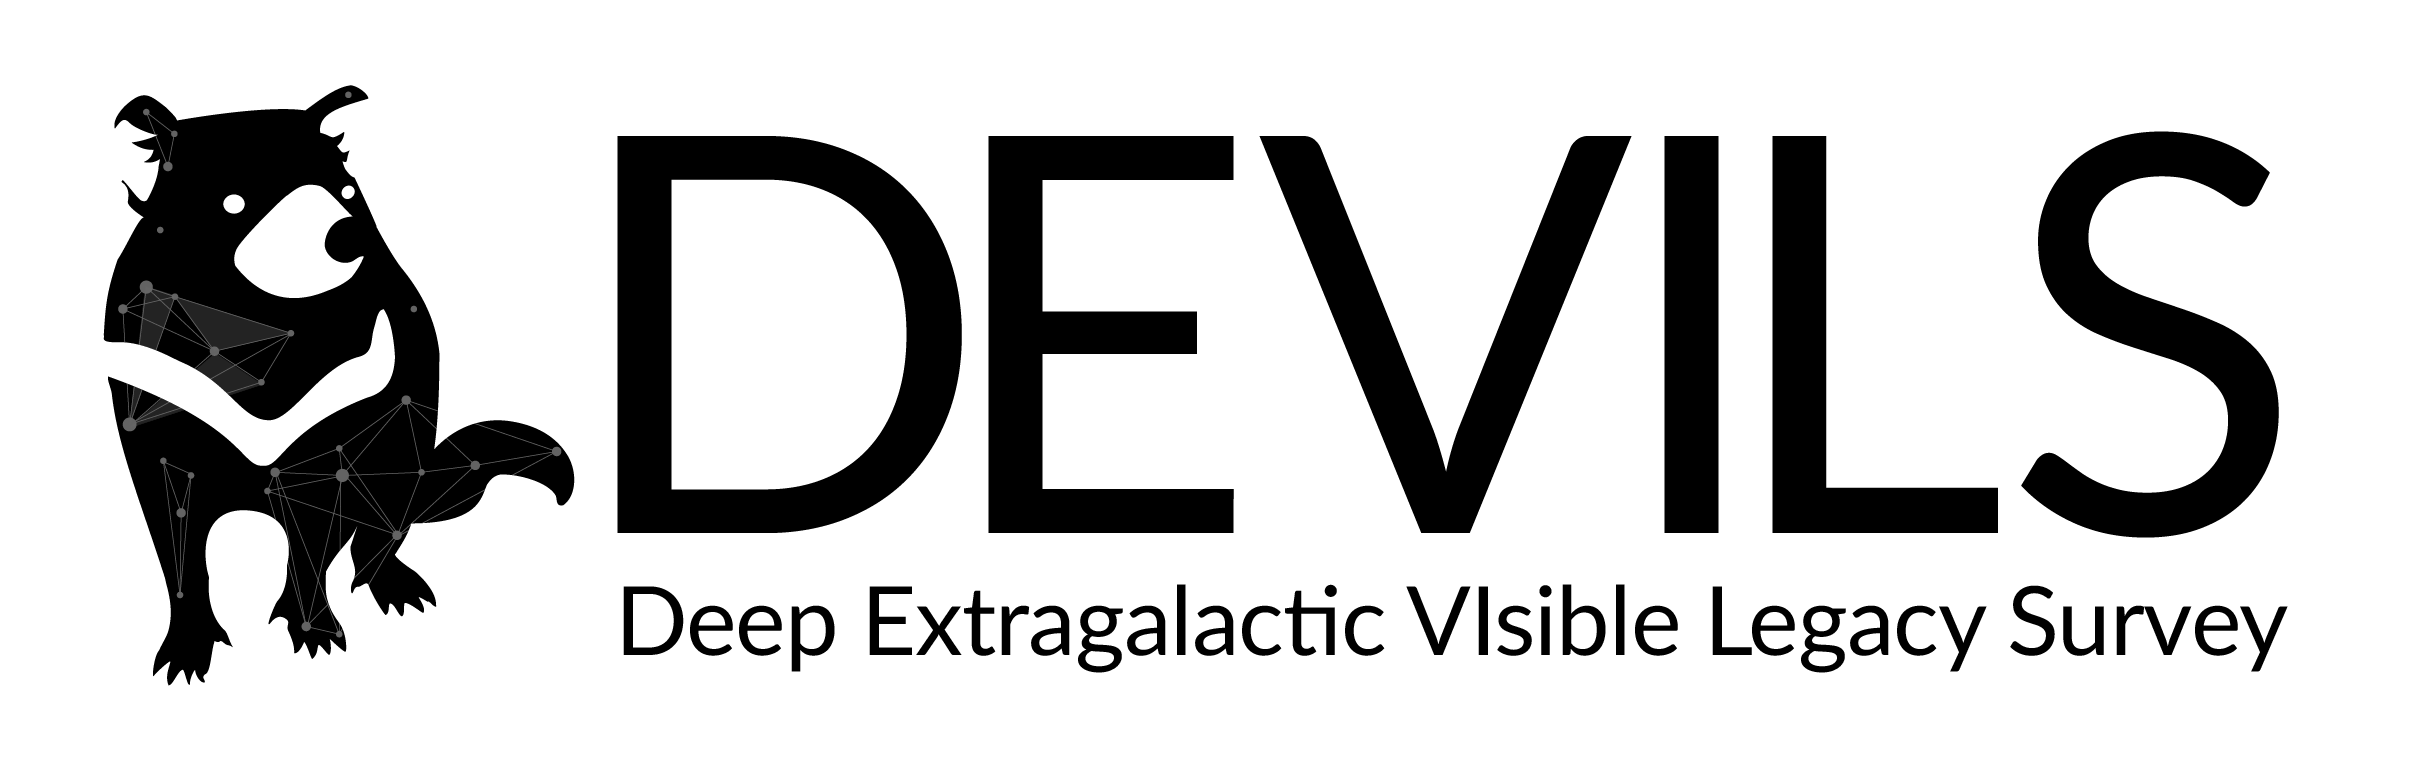
\includegraphics[scale=0.8]{devils-logo_big.png}
\end{center}
\end{figure}

\begin{center}
\Huge {\textcolor{PineGreen}{\textbf{Tool for Analysis and Redshifting (TAZ)}}}\\
\Huge {\textcolor{PineGreen}{\textbf{ Version 0.1}}}\\
\Large \textbf{Luke Davies (5/12/2017)}\\
\end{center}
\normalsize


\section{Installation}

Below is a description of how to install the TAZ data reduction and analysis software and associated packages. In the following, \% will be used for a terminal prompt and $>$ for a prompt in R. For example, where running the the first line given below in Section 1.1.1 only type \texttt{R} not \texttt{\% R}. 

\subsection{External Packages}

There are three main pieces of external software required to run \textsc{taz}. They are i) main coding language \textsc{r}, ii) the 2dfDR data reduction software provided by the the AAO, iii) the AAT targeting/fibre assignment software \textsc{configure}. 

\subsubsection{Installing R}

You can download the version of \textsc{r} specific to your operating systems and via your closest mirror here: \url{https://cran.r-project.org/mirrors.html}. Follow the instructions to install \textsc{r}. You can then check that \textsc{r} is installed correctly, by opening a terminal window and typing: \\


\hspace{10mm} \% R\\

If an \textsc{r} session starts in your terminal you are up and working fine.

\subsubsection{Installing 2dfDR}

The 2dfDR software is used to reduce data from the 2df+AAOmega system at the AAT. You can find detailed information regarding the processes in 2dfDR here:  \url{https://www.aao.gov.au/get/document/2dF-AAOmega-obs-manual-69-88.pdf}.  \\

\textsf{1.1.2.1 Download and Installation} \\

In order to install 2dfDR go here: https: //www.aao.gov.au/science/software/2dfdr and download the appropriate version for your operating system. Note, if you are using Mac OS Sierra, the El Capitan build will likely work fine. If you have issues installing 2dfDR contact AAO support. \\

Once you have downloaded 2dfDR, follow the installation instructions for installation here: \url{https://www.aao.gov.au/science/software/2dfdr/quick-guide}. If you cannot access the installation instructions, the steps are briefly: \\

The file will have a name something like: 2dfdr-linux-5.33.tgz. Unpack the tar file and extract the software to your chosen software directory:\\

\hspace{10mm} \texttt{\% tar -xvzf 2dfdr-linux-5.33.tgz}\\

To install 2dfDR, add the full directory pathname of 2dfdr\_install/bin to your PATH (ensuring that you do not have the environmental variables DRCONTROL\_DIR or DRCONTROL\_ENV already set). To do this: \\

    $\bullet$ In tcsh (set in .tcshrc (or .cshrc if not found)) \\
   \hspace{10mm} \texttt{set path = (\$path /path/to/software/2dfdr\_install/bin)}\\

     $\bullet$ In bash (set in .bash\_profile) \\
    \hspace{10mm} \texttt{export PATH=/path/to/software/2dfdr\_install/bin:\$PATH}\\

     $\bullet$ In csh (set in .cshrc)\\
    \hspace{10mm} \texttt{setenv PATH \$PATH\textbackslash:/path/to/software/2dfdr\_install/bin}\\


where `2dfdr\_install' will be something like `2dfdr-6.46-MacOsX\_ElCapitan'. Note that this is specific to your system environment and may be different from above. \\

Helpful hint: you will need to re-load your shell profile once you have edited it. $e.g.$, for a bash shell with .bash\_profile \\ 

 \hspace{10mm} \texttt{\% source$\sim$/.bash\_profile}\\

to reload. \\

\textsf{1.1.2.2 Check Installation} \\

For running \textsc{TAZ} we use the command line version of 2dfDR called \textsc{aaorun}. To check this is running correctly, open a terminal and type: \\

\hspace{10mm} \% aaorun help\\

This should display the  \textsc{aaorun} command line options. You can also test the 2dfDR GUI software interface is working, but typing: \\

 
\hspace{10mm} \% drcontrol\\

This should give you a nice image of Saturn and tell you that there are no raw data files in your current directory.

\subsubsection{Installing CONFIGURE}

The AAT uses a piece of software called \textsc{configure} to determine fibre assignments and produce the files required to drive 2df. You can find out about what \textsc{configure} does here: \url{https://www.aao.gov.au/science/software/configure}. 

\textsf{1.1.2.1 Download and Installation} \\

On the AAO configue page follow the online instructions for installing configure. For this you will need to go to the AAO ftp site and find the latest version (\url{ftp://ftp.aao.gov.au/pub/2df/configure}). While you are doing this, also download the latest version of the latest version of the astrometry files here: \url{ftp://site-ftp.aao.gov.au/pub/local/2df/latest_config_files}. The Tiling software included in TAZ will actually look-for and download the latest version of these files, but it is good to have the most up-to-date version when starting.  \\



Once again, if you cannot access the installation instructions the steps are briefly: \\

The file will have a name something like: configure-8.4-MacOsX\_ElCapitan\_x86\_64.tar.gz. Unpack the tar file and extract the software to your chosen software directory:\\

\hspace{10mm} \texttt{\% tar -xvzf configure-8.4-MacOsX\_ElCapitan\_x86\_64.tar.gz}\\

You then need to add the full directory to your PATH as will 2dfDR: \\


    $\bullet$ In tcsh (set in .tcshrc (or .cshrc if not found)) \\
   \hspace{10mm} \texttt{set path = (\$path /path/to/software/configure\_install)}\\

     $\bullet$ In bash (set in .bash\_profile) \\
    \hspace{10mm} \texttt{export PATH=/path/to/software/configure\_install/:\$PATH}\\

     $\bullet$ In csh (set in .cshrc)\\
    \hspace{10mm} \texttt{setenv PATH \$PATH\textbackslash:/path/to/software/configure\_install}\\

where `configure\_install' will be something like `configure-8.4-MacOsX\_ElCapitan\_x86\_64'.\\

You will now also have to copy the the most up-to-date version of the astrometry files you downloaded to the \textbf{data\_files} folder in the configure directory:\\

 
\hspace{10mm} \texttt{\% cp  latest\_config\_files/*  /path/to/software/configure\_install/data\_files/}\\


Finally you will need to set the a \texttt{CONFIG\_FILES } environmental variable for \textsc{configure}'s data files:\\

    $\bullet$ In tcsh (set in .tcshrc (or .cshrc if not found)) \\
   \hspace{10mm} \texttt{set CONFIG\_FILES = /path/to/software/configure\_install/data\_files}\\

     $\bullet$ In bash (set in .bash\_profile) \\
    \hspace{10mm} \texttt{export CONFIG\_FILES =/path/to/software/configure\_install/data\_files}\\

     $\bullet$ In csh (set in .cshrc)\\
    \hspace{10mm} \texttt{setenv CONFIG\_FILES /path/to/software/configure\_install/data\_files}\\

$i.e.$ for csh this looks something like:\\ 

\hspace{10mm}  setenv CONFIG\_FILES /Applications/configure-8.4-MacOsX\_ElCapitan\_x86\_64/data\_files/\\


Once agin remember to re-load your shell profile once you have edited it!\\

\textsf{1.1.2.2 Check Installation} \\

You can then check that \textsc{configure} is running correctly by opening a terminal and typing: \\

\hspace{10mm} \% configure\\

You should get a pop-up GUI asking which instrument you are using. Don't worry about this, you should not need to do things manually, but \textsc{TAZ} will now be able to call \textsc{configure} to allocate fibres for observing.

\subsection{Installing R packages}


There are a number of R packages that need to be installed. To do this you should just be able to run the \textsc{InstallTAZ.R} script provided \url{https://github.com/ICRAR/DEVILS-TAZ/blob/master/InstallTAZ.R}. First download the script, then move to the directory where InstallTAZ.R is located, open an R session in a terminal, using:\\

\hspace{10mm} \% R\\

then run:\\

\hspace{10mm}  \texttt{$>$ source(`InstallTAZ.R')}\\

This will install all of the required packages required to run \textsc{TAZ}. You will be asked to select a `CRAN mirror' and a pop-up will appear. Just select the geographically closest location to you. Once this has finished,  ss a quick test of the installation, type:\\

\hspace{10mm}  \texttt{$>$ installed.packages()}\\

and you should see DEVILSTAZ on this list.

\section{Setting Up the DEVILS Directory Structure}

The first stage in running \textsc{TAZ} is to set up the the DEVILS directory structure. To do this, run the \textsc{setUpDir()} function. This function will create the directory structure including all of the calibrations, IDX files (parameters for 2dfDR), and observability plots/logs for each night you are observing.  To run this structure, you will need to input the run and night range for which you wish to generate the data structure for. First open an R session. Then you will need to load the \textsc{DEVILSTAZ} package (this should be all you need to load whenever you start R):\\

\hspace{10mm}  \texttt{$>$ library(`DEVILSTAZ')}\\

The \textsc{setUpDir()}  function is then run as:\\

\hspace{10mm}  \texttt{$>$ setUpDir(workingDir=`.', runs=c(`run1\_2017\_12',`run2\_2018\_01'), \\ dateStart=c(`2017\_12\_18',`2018\_01\_09'),dateEnd=c(`2017\_12\_26',`2018\_01\_22')) }\\


where, \\

 \texttt{workingDir}=directory location you wish to build this structure.\\
 \texttt{runs}=the run names. They must have this format. If you do not know the run you are on, ask Luke (luke.j.davies@uwa.edu.au).\\
 \texttt{dateStart}=First night of each run in year\_month\_day format\\
 \texttt{dateEnd}=Last night of each run in year\_month\_day format\\

Try running this code and explore the directory structure. You can generate this structure for any dates you like. You should have something like:\\

\hspace{5mm} \textbf{data/} 
\vspace{1mm}

\hspace{10mm} \textbf{biases/}
\vspace{1mm}

\hspace{15mm} \textbf{run1\_2017\_12/, ....} 
\vspace{1mm}

\hspace{10mm} \textbf{calibrators/} 
\vspace{1mm}

\hspace{15mm} \textbf{AutoZTemp/} 
\vspace{1mm}

\hspace{15mm} \textbf{filters/} 
\vspace{1mm}

\hspace{15mm} \textbf{GuideStars/}
\vspace{1mm}

\hspace{15mm} \textbf{sensfuncs/}
\vspace{1mm}

\hspace{15mm} \textbf{SkyFibres/}
\vspace{1mm}

\hspace{15mm} \textbf{stdstars/}
\vspace{1mm}

\hspace{10mm} \textbf{darks/} 
\vspace{1mm}

\hspace{15mm} \textbf{run1\_2017\_12/, ....}
\vspace{1mm}

\hspace{10mm} \textbf{idxFiles/} 
\vspace{1mm}

\hspace{10mm} \textbf{logs/} 
\vspace{1mm}

\hspace{10mm} \textbf{observing/} 
\vspace{1mm}

\hspace{15mm} \textbf{D10\_yrPlan2017.png, ....} 
\vspace{1mm}

\hspace{15mm} \textbf{run1\_2017\_12/, ....} 
\vspace{1mm}

\hspace{30mm} \textbf{2017\_12\_18/, ....}
\vspace{1mm}

\hspace{10mm} \textbf{raw/} 
\vspace{1mm}

\hspace{15mm} \textbf{run1\_2017\_12/, ....} 
\vspace{1mm}

\hspace{30mm} \textbf{2017\_12\_18/, ....} 
\vspace{1mm}

\hspace{10mm} \textbf{reduced/}
\vspace{1mm}

\hspace{15mm} \textbf{run1\_2017\_12/, ....} 
\vspace{1mm}

\hspace{30mm} \textbf{2017\_12\_18/, ....} \\

You will populate the \textbf{biases/}, \textbf{darks/}, and \textbf{raw/} part of this structure with the data taken at the AAT, and TAZ will generate reduced data and analysis products in the other parts of the structure.  


\section{Adding Observations}

When observing you will add raw data files to this directory structure. Firstly, at the start of each run, bias and dark frames will be taken. These need to be added to the \textbf{biases/*runName*} and \textbf{darks/*runName*} directories, where *runName* is something like `run1\_2017\_12'. Note that TAZ will aim to generate a master bias and master dark for all files in this directory, so if there are files that you do not wish to be used in making the master darks/biases please keep them in the  \textbf{biases/*runName*/junk/} or \textbf{darks/*runName*/junk/} sub folders.

Next you will need to place the raw target data in the relevant directory. This should be easily done as the date is in the file name produced by the AAT. Data for each night observed should be copied to the relevant \textbf{raw/*runName*/YYYY\_MM\_DD} directory ($i.e.$ for the first observing night on the 18th of December 2017, the data should be copied to \textbf{raw/run1\_2017\_12/2017\_12\_18}). Once again, TAZ will reduce/analyse all data in this directory. So if there are files you do not wish to be included, add then to the \textbf{raw/*runName*/YYYY\_MM\_DD/junk} folder. You do not need to separate ARC, FLAT and TARGET files in this directory. TAZ will identify and match the correct files based on the configuration used in the FITS header.  

For now, there is an example small dataset you can get from here \url{https://www.dropbox.com/s/yutdugiwpi4jo3x/TAZRawExample.zip?dl=0}. Once you have this copy the biases, darks and raw data files to your \textbf{biases/}, \textbf{darks/}, and \textbf{raw/} folders under the correct run/date.  

\section{Running TAZ}

Here I will just give a high level overview of running the TAZ software. More detailed descriptions of the individual functions can be accessed via the R help functions by simply opening an R terminal and typing: \\

\hspace{10mm}  \texttt{$>$ ?*FUNCTION\_NAME*}\\

for example, to get an overview of the main high-level \texttt{TAZ} function, type:\\

\hspace{10mm}  \texttt{$>$ ?TAZ}\\

In most cases this code will by run end to end with one line. However, here I split it into various sections to explain what the code is doing and to allow the user to run each component separately. Note that parts of TAZ can be run in a a parallel fashion, to use this set the \texttt{cores} key word in the TAZ command line.

\subsection{Running the 2dfDR reduction}

First, lets try and run TAZ on our test dataset to just perform the data reduction. To do this, make sure you are in the directory above the \textbf{/data} directory you just generated, and run:\\

\hspace{10mm} \texttt{$>$ TAZ(user='NewUser', workingDir='.', verbose=2, doReduce=T, doExtract=F, doStack=F, doAutoZ=F, cores=2, doUpdateMaster=F, doTiler=F, zeroPoint=T)}\\

This should run TAZ over your current directory, reducing the data using 2dfDR. TAZ will automatically look for data that have not been reduced in your directory structure. It does this by identifying run/date folders there there is raw data, but nothing in the corresponding \textbf{reduced/.../.../} folder. You can force TAZ to reduce (or re-reduce) data from a given night or nights (see next section). However, note that this will overwrite the current reduction for that night, so use with care. 

When the code has finished running the command given above, you should find that some of the \textbf{data/reduced/} sub-folders are populated. Check that this is the case. The most important thing to check is that you have reduced files in the \textbf{data/reduced/run1\_2017\_12/ \\ 2017\_12\_18/} folder.  If not, go back and check you followed the previous stages correctly, and if you are still experiencing problems contact Luke.  

One additional option is available at this stage which will produce diagnostic plots of all bias and dark frames you are using to make the MASTER bias and dark. This is very useful for quality control and checking observations at the telescope. To do this simply add \texttt{doCalibQC=F} to the line running TAZ. This will produce plots in both \textbf{/data/darks/run\#\_YYYY\_YY/} and \textbf{/data/biases/run\#\_YYYY\_YY/} to aid in QC of the calibration files.

\subsection{Running the 2dfDR reduction on a specific directory}

TAZ has the functionality to run a 2dfDR reduction on data from a specific night alone. To do this, simply set the \texttt{toReduceDirs} keyword in the command line. This variable will need to be passed a string vector containing the path to the nights you wish to reduce (or re-reduce). You can do this as: \\


\hspace{10mm} \texttt{$>$ toReduceDirs<-`data/rawdata/run1\_2017\_12/2017\_12\_18'}\\
\hspace{10mm} \texttt{$>$ TAZ(user='NewUser', workingDir='.', verbose=2, doReduce=T, toReduceDirs=toReduceDirs, doExtract=F, doStack=F, doAutoZ=F, cores=2, doUpdateMaster=F, doTiler=F, zeroPoint=T)}\\

Try this now and you will see that the reduced data in \textbf{data/reduced/run1\_2017\_12/2017\_12\_18} has been over written. In practice, it is suggested you only use this functionality if you know what you are doing!
 

\subsection{Running the 2dfDR reduction and 1D extraction}

Next we can try and run both a reduction and extract 1D spectra from each of our reduced frames. As TAZ looks for directories that have already been reduced, you will need to delete the products you have previously made in the \textbf{/data/reduced/run1\_2017\_12/2017\_12\_18/} and \textbf{/data/reduced/run1\_2017\_12/ \\ 2017\_12\_19/} directories, before rerunning this code. To do the reduction and extraction simply set \texttt{doExtract=T} and run:\\

\hspace{10mm} \texttt{$>$ TAZ(user='NewUser', workingDir='.', verbose=2, doReduce=T, doExtract=T, doStack=F, doAutoZ=F, cores=2, doUpdateMaster=F, doTiler=F, zeroPoint=T)}\\

This should run TAZ over you current directory, reduce the data using 2dfDR AND extract 1D spectra. The most important thing to check is that you have individually reduced spectra in the `.Rdata' format in the \textbf{data/reduced/allSpec/} directory. If not, go back and check you followed the previous stages correctly, and if you are still experiencing problems contact Luke.  \\

As you may not want to re-run the reduction, you can tell TAZ to skip this part of the pipeline. However, you then have to tell TAZ which files to extract 1D spectra from. This is achieved by setting  \texttt{doReduce=F} and then adding the variable: \texttt{toExtractFiles=*a string list of files to extract*}. In our example, this would be:\\

 \hspace{10mm} \texttt{$>$ toExtractFiles<-c(`data/reduced/run1\_2017\_12/2017\_12\_18/ \\ 2017\_12\_18\_config\_1\_reduced.fits', `data/reduced/run1\_2017\_12/2017\_12\_19/ \\ 2017\_12\_19\_config\_1\_reduced.fits')}\\
 
  \hspace{10mm} \texttt{$>$ TAZ(user='NewUser', workingDir='.', verbose=2, doReduce=F, doExtract=T, toExtractFiles=toExtractFiles, doStack=F, doAutoZ=F, cores=2, \\ doUpdateMaster=F, doTiler=F, zeroPoint=T)}\\

 This will skip the reduction phase and extract 1D spectra from the reduced files provided.
 
 \subsection{Stacking extracted spectra}
 
 As DEVILS will observe the same spectra over multiple observations, these will need to be stacked to increase single to noise. TAZ can perform this stacking from previously extracted spectra (as above). As TAZ writes all reduced spectra to the \textbf{/data/reduced/allSpec/} directory, the staking procedure simply searches for all instances of a particular ID in this directory and inverse variance weights the spliced spectrum, individual CCD arms and continuum extracted spectra. As we do not wish to extract the spectra again, set \texttt{doExtract=F} and \texttt{doStack=T}. Once again, in order to run this, you must tell TAZ which IDs to stack. This can either be done by providing a vector list of IDs (note our example data is from GAMA and all objects are appended with a 'G", in DEVILS this will be 'D'):\\
 
   \hspace{10mm} \texttt{$>$ toStackIDs<-c(`G006014', 'G006158')}\\
 
  \hspace{10mm} \texttt{$>$ TAZ(user='NewUser', workingDir='.', verbose=2, doReduce=F, doExtract=F, doStack=T,  toStackIDs=toStackIDs, doAutoZ=F, cores=2, doUpdateMaster=F, \\ doTiler=F, zeroPoint=T)}\\ 
  
 A second option is to tell TAZ to try and stack all IDs in the current \textbf{/allSpec} folder. To do this, simply set the \texttt{toStackIDs} value to `all': \\
  

  \hspace{10mm} \texttt{$>$ TAZ(user='NewUser', workingDir='.', verbose=2, doReduce=F, doExtract=F, doStack=T,  toStackIDs='all', doAutoZ=F, cores=2, doUpdateMaster=F, doTiler=F, zeroPoint=T)}\\   

Run this code now. TAZ should populate the \textbf{/data/reduced/stackedSpec/} folder of your directory structure with 1D spectra. You can now quickly look at one of these spectra manually to see this has worked, in R do:\\

\hspace{10mm} \texttt{$>$ load(`data/reduced/stackedSpec/G006158.Rdata')} \\

\hspace{10mm} \texttt{$>$ magplot(spec\$wave, spec\$flux, type='l')} \\

and over-plot the blue and red arms separately:\\


\hspace{10mm} \texttt{$>$ lines(spec\$waveBlue, spec\$fluxBlue, col='blue')}\\

\hspace{10mm} \texttt{$>$ lines(spec\$waveRed, spec\$fluxRed, col='red')}\\

or plot the continuum extracted stacked spectrum:\\

\hspace{10mm} \texttt{$>$ magplot(spec\$wave,spec\$fluxSub, type='l')}\\

Or better you could simply run:\\

\hspace{10mm} \texttt{$>$ specPlot(spec)}\\

\texttt{specPlot()} is a TAZ function that allows easily plotting of the spectral structures output by TAZ. Try this now. If you want to see all information available for this spectrum, simply type:\\

 \hspace{10mm} \texttt{$>$ names(spec)} \\
 
 and then your chosen parameter, $i.e.$:\\
 
 
  \hspace{10mm} \texttt{$>$ spec\$EXP} \\
  
 If you look at the spec\$z parameter, it will not currently have a value. This is because we haven't yet measured a redshift.....
 

 \subsection{Running AutoZ on Stacked Spectra}
 
 Next we will run AutoZ over all of our stacked spectra. This is done by setting the \texttt{doAutoZ=T} flag. As we do not wish to stack the spectra again, we will set \texttt{doStack=F}. Once again, in order to run this, you must tell TAZ which stacked spectra to run AutoZ over. This can either be done by providing a vector list of file locations. \\
 
 \hspace{10mm} \texttt{$>$ toAutoZStacks<-c(`data/reduced/stackedSpec/G006014.Rdata',  \\ 'data/reduced/stackedSpec/G006158.Rdata')}\\
 
 \hspace{10mm} \texttt{$>$ TAZ(user='NewUser', workingDir='.', verbose=2, doReduce=F, doExtract=F, doStack=F,  doAutoZ=T, toAutoZStacks=toAutoZStacks, cores=2, doUpdateMaster=F, doTiler=F, zeroPoint=T)}\\ 
 
Or as for the stacking, you can also tell TAZ to try and run AutoZ for all IDs in the current \textbf{/stackedSpec/} folder. To do this, simply set the \texttt{toAutoZStacks} value to `all': \\
  

  \hspace{10mm} \texttt{$>$ TAZ(user='NewUser', workingDir='.', verbose=2, doReduce=F, doExtract=F, doStack=F, doAutoZ=T,  toAutoZStacks=`all',  cores=2, doUpdateMaster=F, \\ doTiler=F, zeroPoint=T)}\\  
  
This should run AutoZ over all spectra in the \textbf{/stackedSpec/} folder. Do this now. You should find that the code populates the \textbf{/data/reduced/stackedSpec/AutoZplots/} folder with figures. These are the same ones as produced by \texttt{plotSpec()}. The code is also updating the meta information in all of the individual spectra `.Rdata' files in \textbf{/data/reduced/stackedSpec/}. If you now reload the spectrum above, you will find it has a redshift and a probability that that redshift is correct:\\  

\hspace{10mm} \texttt{$>$ load(`data/reduced/stackedSpec/G006158.Rdata')} \\

\hspace{10mm} \texttt{$>$ spec\$z} \\

\hspace{10mm} \texttt{0.7750067}\\
 
 \hspace{10mm} \texttt{$>$ spec\$prob} \\
 
 \hspace{10mm} \texttt{0.5725674}\\

TAZ will also make plots of all of the sources you have run AutoZ over in the \textbf{/data/reduced/stackedSpec/ AutoZplots/}. The spectrum for G006158 can be seen in Figure \ref{fig:specEx}. These figures are useful for checking quality control during observations and for examining TAZ outputs.

\begin{figure}
\begin{center}
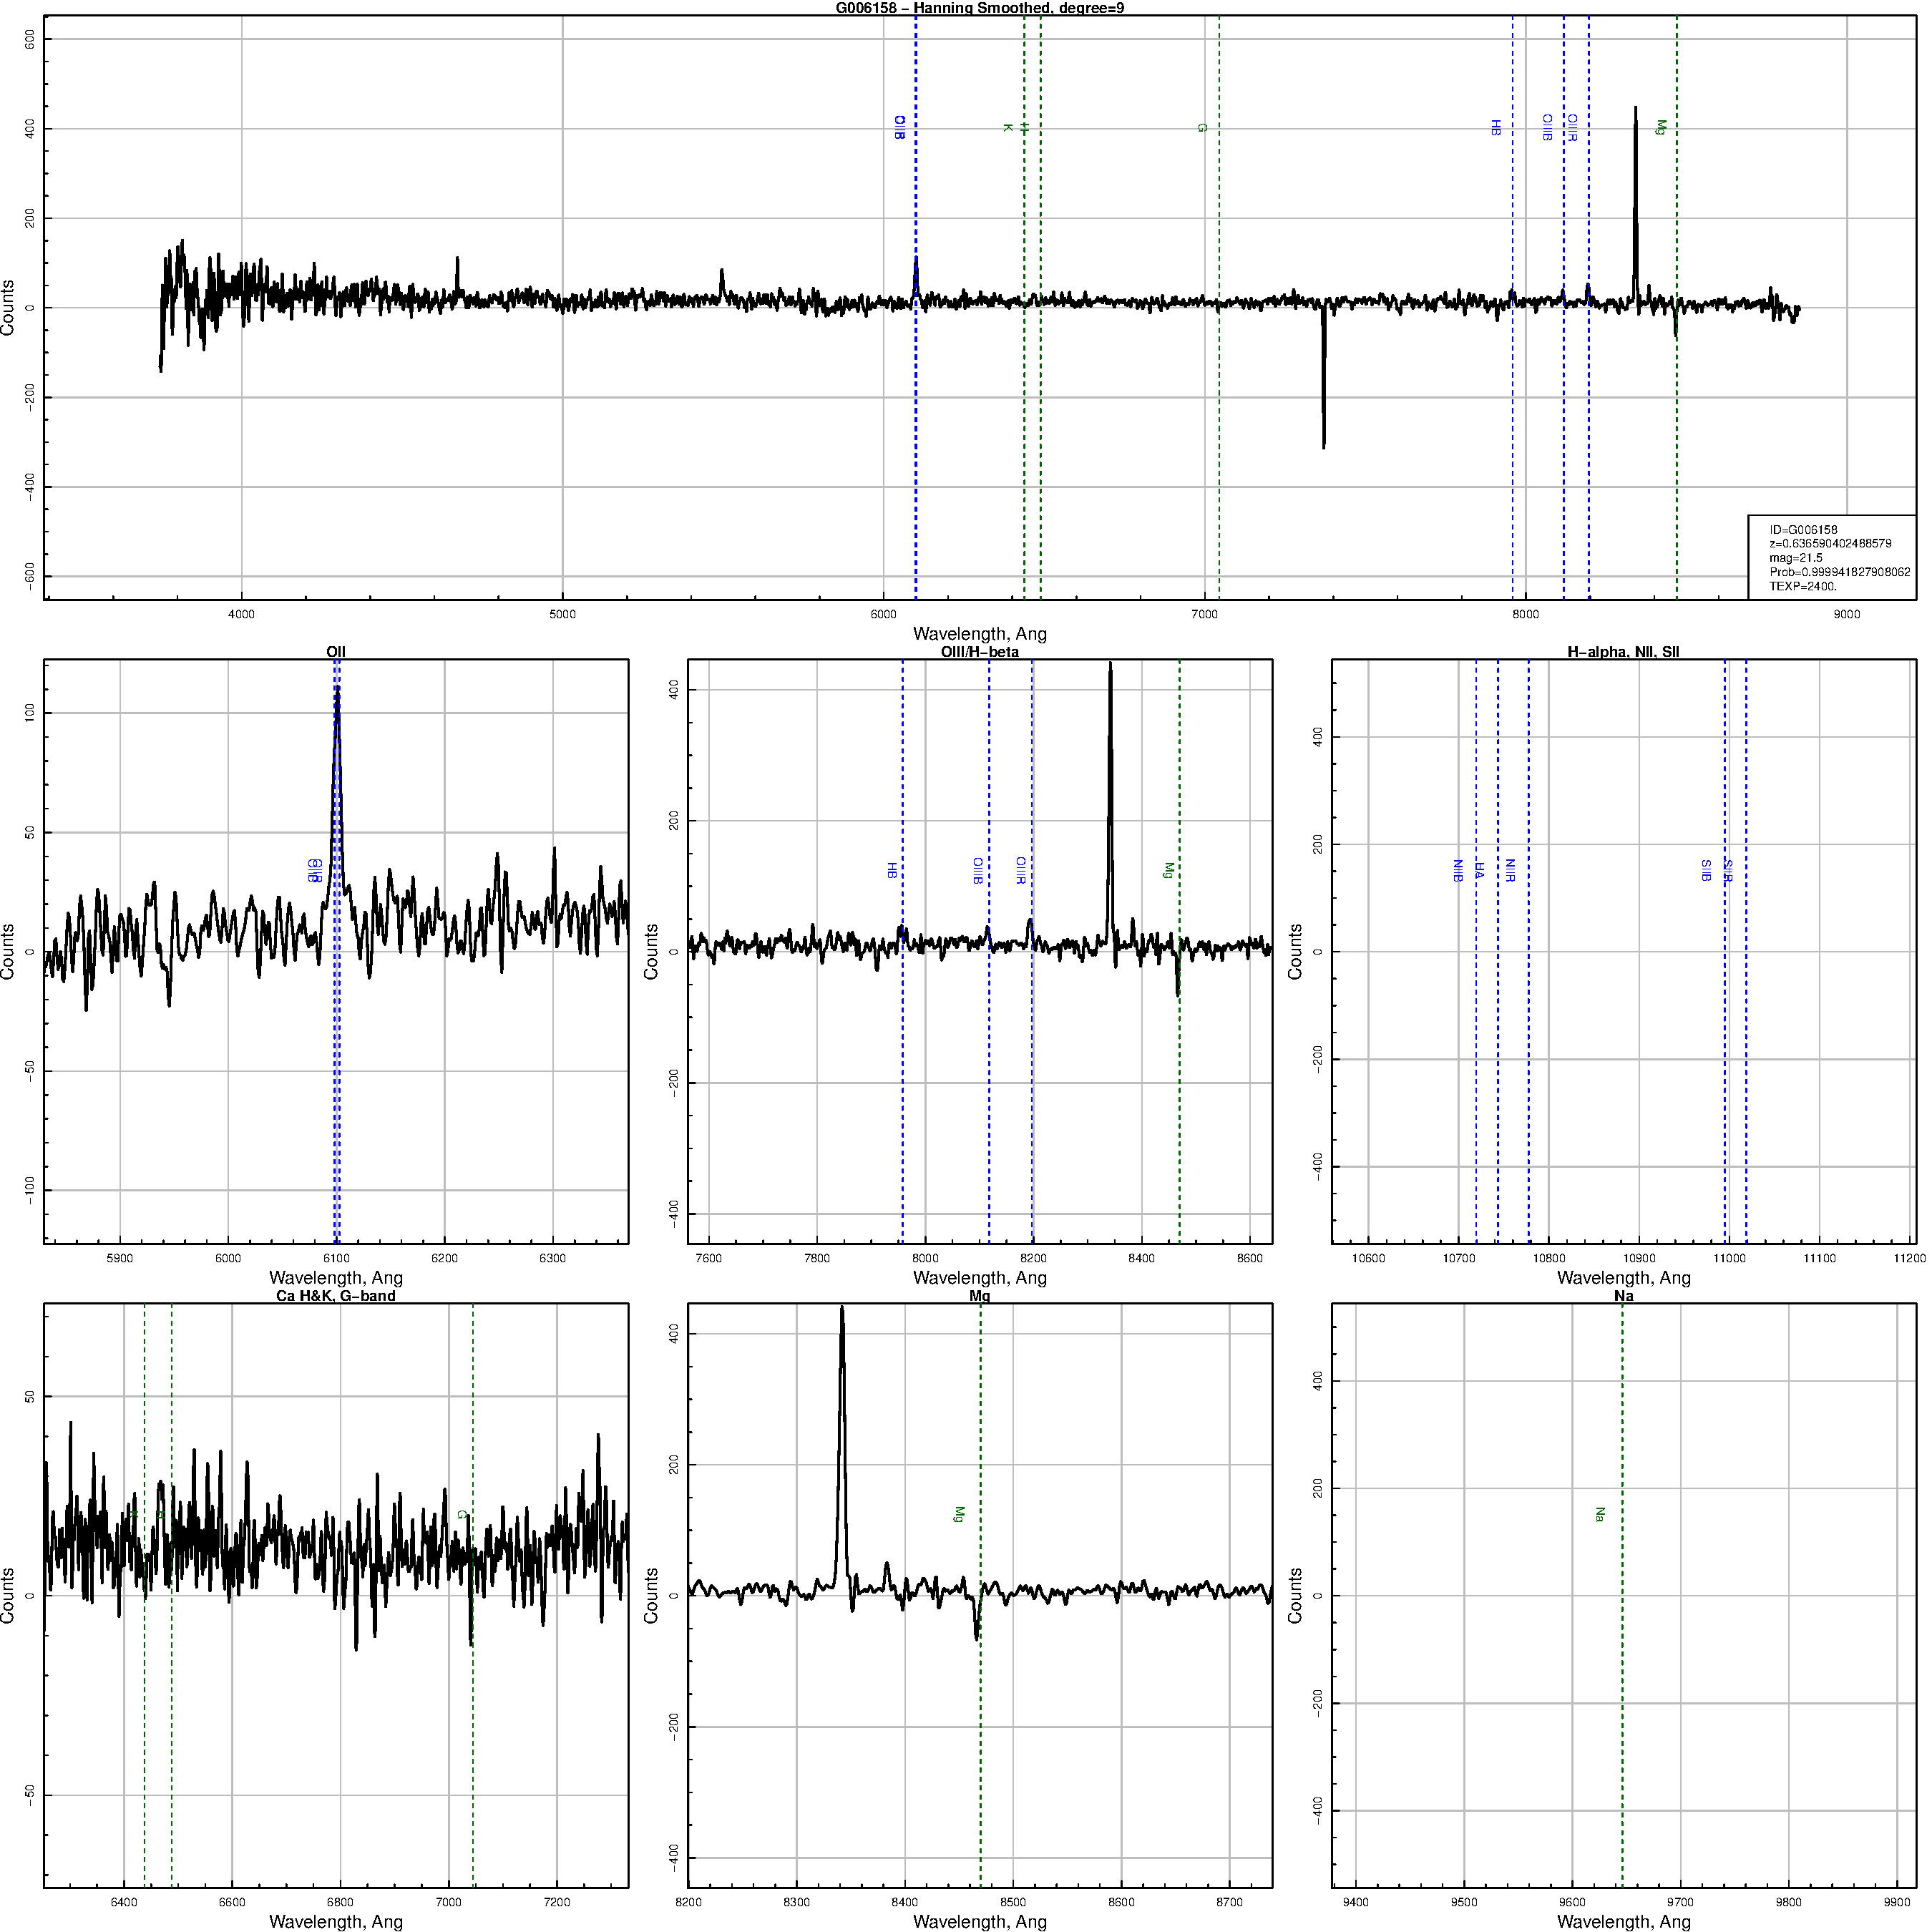
\includegraphics[scale=0.4]{G006158.pdf}
\caption{Example output of TAZ after running AutoZ. Top row shows the full spectrum, middle row shows the location of key emission features at the source's measured redshift, and the bottom row shows the same but for absorption features. Line positions at the fitted redshift are shown as dashed vertical lines (emission in blue and absorption in green). Details of the fitted redshift are given in the legend of the top panel. All spectra are Hanning smoothed.}
\label{fig:specEx}
\end{center}
\end{figure}


 \subsection{Updating Master Catalogues with new redshifts and producing new observing catalogues}

Once we have now redshifts, we will wish to update our master catalogues to reflect this, and produce new observing catalogues with updated priorities. In TAZ this is done by setting \texttt{doUpdateMaster=T}. If set, TAZ will:\\

$\bullet$ Find the most recent DEVILS Master Catalogue (DMCat) in the \textbf{data/catalogues/MASTERcats} directory.\\


$\bullet$ Read all of the spectra in the \textbf{/data/reduced/stackedSpec/} directory and update the DEVILS\_z,  DEVILS\_prob,..... values in the catalogue.\\

$\bullet$ Save a new DMCat to \textbf{/data/catalogues/MASTERcats/} with the current date. \\

$\bullet$ Identify the next observing date in your current directory structure (past the date you are running the code) and create a DEVILS observing catalogues (DOCats) directory here \textbf{data/observing/run\#\_YYYY \_MM/YYYY\_MM\_DD/DOCats}. Within this file all of the target, guide, sky, standards catalogues that are required for the Tiling configuration are produced.\\

To generate to do this simply set \texttt{doUpdateMaster=T} run:\\

  \hspace{10mm} \texttt{$>$ TAZ(user='NewUser', workingDir='.', verbose=2, doReduce=F, doExtract=F, doStack=F, doAutoZ=F,  cores=2, doUpdateMaster=T, doTiler=F, zeroPoint=T)}\\  
  
  Check that TAZ produces the relevant files. 


 \subsection{Producing new fibre configuration files}
 
 The final part of TAZ is to generate new fibre configuration files for the next night's observing. This is done by first setting \texttt{doTiler=T}. One important extra parameter that needs to be set for this function to work, is the location of the directory containing the AAT's \textsc{configure} software, that was installed at the start of this document. To do this simply add the directory location as the \texttt{confidir} parameter in TAZ. For modern Macs (and the default) this will be something like: \texttt{configdir=`/Applications/configure-8.4-MacOsX\_ElCapitan\_x86\_64'}. You will also need to tell TAZ which DO catalogues directory to use in the \texttt{DODir} parameter. Finally, we also need to tell TAZ how many fibre allocation files to make in each filed, and whether to start on plate 0 or 1 of 2dF. This is done in the following way: \\
 
  \hspace{10mm} \texttt{$>$ TAZ(user='NewUser', workingDir='.', verbose=2, doReduce=F, doExtract=F, doStack=F, doAutoZ=F, doUpdateMaster=F, doTiler=T, DODir='data/observing/run 1\_2017\_12/2017\_12\_20/DOCats', zeroPoint=T,  cores=4,  N\_D02A=1,N\_D02B=1, N\_D03=1, N\_D10=1, D02A\_startPlate=0, D02B\_startPlate=1, D03\_startPlate=0, D10\_startPlate =1)}\\  
 
 The final parameters of this line tell TAZ to produce 1 configuration in each of D02A, D02B, D03, and D10, and to start on plate 0 for D02A, 1 for D02B, 0 for D03 and 1 for D10. You can try and run this code now. Be aware that this will take some time. TAZ will generate the configuration files on one core per field if \texttt{cores}$>$3. 
 
 Within the supplied DOcats directory, TAZ will produce a sub-folder called \textbf{Tiling}, within this there will be one sub-folder per field requested, and in this one folder for each configuration, called \textbf{TargetFork....}. These files contain the .fld and .sds files produced by \textsc{configure} and needed to assign fibres on 2dF. All of these files are date-stamped and copied to a directory called  \textbf{Tiling/TilesFiles}  so that they can be provided to the support astronomer for the next night's observing (see the DEVILS\_Observing\_Manual.pdf for further details). 
 
 
 \subsection{Putting it all together}
 
 TAZ functions are rarely run in isolation as above. In practice, at the end of each night's observing the full code will be run end to end. This can be achieved by running something like: \\
 
  \hspace{10mm} \texttt{$>$  TAZ(user='NewUser', workingDir=''.'', verbose=2,  doCalibQC=F, doReduce =T, doExtract=T, doStack=T,  doAutoZ=T,  doUpdateMaster=T, doTiler=T, zeroPoint =T, cores=4, configdir='/Applications/configure-8.4-MacOsX\_ElCapitan\_x86\_64' N\_D02A=0,N\_D02B=0, N\_D03=3, N\_D10=3, D02A\_startPlate=0, D02B\_startPlate=0, D03 \_startPlate=0, D10\_startPlate=1)}\\

This will run the full reduction and analysis pipeline from end to end using 4 cores. It will then produce three fibre configurations in D03 starting on plate 0 and three configurations in D10 starting on plate 1. If you want to run the pipeline from end to end on the test dataset. Make sure you delete the reduced data in each of the  \textbf{/data/reduced/run\#\_YYYY\_MM/ \\ YYYY\_MM\_DD/} directories, otherwise TAZ will not re-reduce them. 

\section{TAZ inputs list}

Below is a list of TAZ inputs and what they do designed to be a reference guide to running TAZ. These can be accessed in \textsc{r} by using the help function ($i.e.$ \texttt{$>$ ?TAZ}):\\


$\bullet$ \texttt{user} - A string identifier which will be added to log files to show who ran the code. \\

$\bullet$ \texttt{workingDir} - The directory location where your previously generated \textbf{data/...} data structure is located.\\

$\bullet$ \texttt{verbose} - How much information to give you about TAZ,  verbose=0,1,2.\\

$\bullet$ \texttt{doReduce} - TRUE/FALSE. Do you want to reduce new data? TAZ will look for new data as files where there is data in the \textbf{raw/} directory for a particular night, but nothing in the corresponding \textbf{reduced/} directory. 

$\bullet$ \texttt{toReduceDirs}  - For the advanced user, you can force this by adding the directory path of nights you with to reduce in the form: data/rawdata/run\#\_YYYY\_MM/YYYY\_MM\_DD (i.e. data/rawdata/run1\_2017\_12/2017\_12\_18). Note that this will overwrite any reduced data in the corresponding \textbf{reduced/} directory ($i.e.$ data/reduced/run1\_2017\_12/2017\_12\_18).    \\

$\bullet$ \texttt{doCalibQC} - TRUE/FALSE. Produce bias/dark QC plots.\\

$\bullet$ \texttt{doExtract} - TRUE/FALSE. Do you want to extract 1D spectra from the files you have reduced? If you have set \texttt{doReduce=F} and \texttt{doExtract=T} you will need to provide a list of reduced files to extract..... \\

$\bullet$ \texttt{toExtractFiles} - A string vector list of reduced files for which you wish to extract 1D spectra. Set if \texttt{doReduce=F} and \texttt{doExtract=T}. These need to be the full directory path in the DEVILS data structure. $i.e.$ data/reduced/run2\_2018\_01/2018\_1\_9/2018\_1\_9\_config\_1\_reduced.fits. \\

$\bullet$ \texttt{doStack} - TRUE/FALSE. Do you want to stack extracted spectra? If you have set \texttt{doExtract=F} and \texttt{doStack=T} you will need to provide a list of spectra IDs to stack..... \\

$\bullet$ \texttt{toStackIDs} - A string vector list of ID for which you wish to stack. Here you just provide the IDs in a string. $I.e.$ D10021811.\\

$\bullet$ \texttt{doAutoZ} - TRUE/FALSE. Do you want to run Auto-z over the stacked spectra? If you have set \texttt{doStack=F} and \texttt{doAutoZ=T} you will need to provide a list of stacked spectra files..... \\

$\bullet$ \texttt{toAutoZStacks} - A string vector list of stacked spectra files for which you wish to run Auto-z. These need to be the full directory path in the DEVILS data structure. $i.e.$ data/reduced/stackedSpec/ D10021811.Rdata. \\

$\bullet$ \texttt{doUpdateMaster} - TRUE/FALSE. Do you want to update the master catalogue with new redshift. This will produce a new master catalogue with the current date (DMcats). And produce the observing catalogues for the next observation data DOcats. \\ 

$\bullet$ \texttt{doTiler} -  TRUE/FALSE. Do you want to generate new tile configurations for the next night of observations? \\

$\bullet$ \texttt{DODir} - If you have set \texttt{doUpdateMaster=F} and \texttt{doTiler=T} you need to tell the code which observation catalogues to use. Set this to a string with the DOCat directory location. Something like: $\sim$DEVILS/TAZ/data/observing/run1\_2017\_12/2017\_12\_18/DOCats/.\\

$\bullet$ \texttt{N\_D?} - Number of new fibre configurations to generate in each field. Use for next night's tiling\\

$\bullet$ \texttt{D?\_startPlate} - Starting plate number for each configuration (either 0 or 1)\\

$\bullet$ \texttt{zeroPoint} -  TRUE/FALSE. Do you want to zero point flux calibrate the spectra? This isn't needed for the redshifting. \\

$\bullet$ \texttt{cores} - Number of core to uses when running the reduction, AutoZ fitting and fibre configuration. \\

$\bullet$ \texttt{configdir} - String containing the directory path location of your installation of the \textsc{configure} software. 



\section{TAZ Outputs list}

TAZ will have generated a large number of output files in different parts of the directory structure. Below is a list of key data products produced by TAZ such that you can easily find things in the data structure: 

\subsection{Raw Data Meta Information:}

\textbf{/data/raw/run\#\_YYYY\_MM/YYYY\_MM\_DD/YYYY\_MM\_DD\_metaData.Rdata} 

R data file containing meta data from FITS header of all raw files in the current directory. To view this data, move to the directory in which is is contained, open and R session and type: \\

\hspace{10mm}  \texttt{$>$ load(`YYYY\_MM\_DD\_metaData.Rdata')}\\

\hspace{10mm}  \texttt{$>$ metaData}\\
  
 
 This will display the filename, ccd, field, RA/DEC centre, exposure time in seconds, the type of data, fibre configuration, date and grating for each file.  

 
\subsection{Spliced reduced data for each night/configuration:} 
 
 \textbf{/data/reduced/run\#\_YYYY\_MM/YYYY\_MM\_DD/YYYY\_MM\_DD\_config\_?\_reduced.fits} 
 
 FITS file with the fully reduced and spliced data for a particular fibre configuration. These are found within the data structure under each night in the \textbf{reduced/} folder. 

  
\subsection{Blue arm reduced data for each night/configuration:} 
   
   \textbf{/data/reduced/run\#\_YYYY\_MM/YYYY\_MM\_DD/ccd1/YYYY\_MM\_DD\_config\_? \\ \_reduced\_blue.fits} 
   
 FITS file with the fully reduced blue data for a particular fibre configuration. These are found within the data structure under each night in the \textbf{reduced/} folder (note that the blue and red arms are in \textbf{ccd1} and \textbf{ccd2} subdirectories). 

 
  
\subsection{Red arm reduced data for each night/configuration:} 
  
  \textbf{/data/reduced/run\#\_YYYY\_MM/YYYY\_MM\_DD/ccd2/YYYY\_MM\_DD\_config\_? \\ \_reduced\_blue.fits} 
  
  FITS file with the fully reduced red data for a particular fibre configuration. These are found within the data structure under each night in the \textbf{reduced/} folder (note that the blue and red arms are in \textbf{ccd1} and \textbf{ccd2} subdirectories). 

 

\subsection{Meta Information for all reduced configurations:} 
 
 \textbf{/data/reduced/run\#\_YYYY\_MM/YYYY\_MM\_DD/YYYY\_MM\_DD\_metaData.Rdata} 
 
 Meta information for all reduced data frames. To view this data, move to the directory in which is is contained, open and R session and type:\\
 

\hspace{10mm}  \texttt{$>$ load(`YYYY\_MM\_DD\_metaData.Rdata')}\\

\hspace{10mm}  \texttt{$>$ metaData}\\

 This will display the filename, ccd, field, RA/DEC centre, exposure time in seconds, the type of data, fibre configuration, date and grating for each file.  
  
 
 \subsection{Flux calibration meta information for each reduced configuration:} 
  
  \textbf{/data/reduced/run\#\_YYYY\_MM/YYYY\_MM\_DD/ccd2/YYYY\_MM\_DD\_config\_? \\ \_reduced\_zeroPoints.Rdata} \\
  
  R data file with flux calibration information for each reduced frame. To view this data, move to the directory in which is is contained, open and R session and type:\\
 

\hspace{10mm}  \texttt{$>$ load(`run\#\_YYYY\_MM/YYYY\_MM\_DD\_config\_?\_reduced\_zeroPoints.Rdata')}\\

\hspace{10mm}  \texttt{$>$ zeroPoints}\\

This will display:\\

ZP - Magnitude zero point of the frame calculated from standard stars     \\
ZPMAD - Median average deviation of ZP    \\
ZPRMS - RMS of ZP   \\
ZPNUM - Number of standards used to calculate ZP\\
FLUXSC - The flux scaling to convert counts to ergs/sec/cm$^2$/Ang/\\
ZP\_red ... - Same values for red and blue arm data individually.  \\


 \subsection{Individual extracted spectra from corresponding reduced configuration/night:}
 
  \textbf{/data/reduced/run\#\_YYYY\_MM/YYYY\_MM\_DD/ccd2/YYYY\_MM\_DD\_config\_? \\ \_reduced\_spec/}\\
   
 Directory containing all individually reduced spectra from the corresponding  configuration. This directory will also contain 1D plots if requested in TAZ. Each spectrum is stored as an R data structure. To view this data, move to the directory in which is is contained, open and R session and type (for example):\\
  
\hspace{10mm}  \texttt{$>$ load(`2017\_12\_18\_G2271755.Rdata')}\\

\hspace{10mm}  \texttt{$>$ spec}\\  

This structure contains various data and meta information for this observation, such a flux, wavelength, sky. It also retains the individual blue and red arms of the spectrum prior to splicing. Note that these are not flux calibrated, but contain the flux calibration information to convert pixels to ergs/sec/cm$^2$/A (fluxSc). To view the spectrum simply type:\\

 \hspace{10mm}  \texttt{$>$ magplot(spec\$wave, spec\$flux, type='l')}\\  

or to list available meta information type:\\

 \hspace{10mm}  \texttt{$>$ names(spec)}\\  

These can be displayed as, $i.e.$:\\

 \hspace{10mm}  \texttt{$>$ spec\$RA}\\ 
 
 All spectra extracted in this way are also copied to the \textbf{data/reduced/allSpec/} directory.


 \subsection{Individual spectra meta information for each configuration/night:} 
 
  \textbf{/data/reduced/run\#\_YYYY\_MM/YYYY\_MM\_DD/ccd2/YYYY\_MM\_DD\_config\_?\_reduced\_meta.Rdata} 
  
 This is an R data file containing the meta information for each spectrum row in the corresponding reduced file. To view this data, move to the directory in which is is contained, open and R session and type:\\
 

\hspace{10mm}  \texttt{$>$ load(`YYYY\_MM\_DD\_config\_?\_reduced\_meta.Rdata')}\\

\hspace{10mm}  \texttt{$>$ meta}\\

This will display:\\

\texttt{ID} - Source ID from input catalogue    \\
\texttt{RA} - Fibre RA \\
\texttt{DEC} - Fibre DEC \\
\texttt{X} - Fibre X \\
\texttt{Y} - Fibre Y \\
\texttt{XERR} - Fibre X error \\
\texttt{YERR}- Fibre Y error\\
\texttt{THETA} - Fibre angle \\
\texttt{TYPE} - Type of source (Target, sky, standard, guide)\\
\texttt{MAG} - Magnitude of source from input cat\\
\texttt{FIBRE} - Fibre Number\\
\texttt{FILE} - The file name and location of the extracted spectrum \\
\texttt{EXP} - The exposure time of the spectrum \\

 \subsection{Individual stacked source spectrum files with redshifts:}
 
  \textbf{data/reduced/stackedSpec/*ID*.Rdata} 
  
  R data structure containing 1D stacked spectra and meta information. This can be accessed as, $i.e.$:
  
  \hspace{10mm}  \texttt{$>$ load(`data/reduced/stackedSpec/G2271755.Rdata')}\\

Available data products can be displayed as:\\

\hspace{10mm}  \texttt{$>$ names(spec)}\\  

These are: \\

\texttt{wave} - vector of wavelength positions from spliced spectrum \\
\texttt{flux} - vector of counts from spliced spectrum \\
\texttt{sn} - vector of variance from spliced spectrum \\
\texttt{sky} - vector of sky values from spliced spectrum \\
\texttt{ID} - ID of spectrum \\
\texttt{RA} - Right Ascension of spectrum, J2000 \\
\texttt{DEC} - Declination of spectrum, J2000 \\ 
\texttt{MAG} - Magnitude of source provided to 2dF \\
\texttt{xunit} - x-axis unit (will be 'ang') \\
\texttt{yunit} - y-axis unit (will be 'ang' - used internally in TAZ and for plotting in package spec.tools) \\
\texttt{z} - redshift of spectrum  \\
\texttt{EXP} - Total exposure time, sec \\
\texttt{NStack} - Number of spectra that went into the stack\\
\texttt{waveBlue} - vector of wavelength positions from blue ccd spectrum\\
\texttt{fluxBlue} - vector of counts from blue ccd spectrum\\
\texttt{snBlue} - vector of variance from blue ccd spectrum\\
\texttt{skyBlue} - vector of sky values from blue ccd spectrum\\
\texttt{waveRed} - vector of wavelength positions from Red ccd spectrum\\
\texttt{fluxRed} - vector of counts from Red ccd spectrum\\
\texttt{snRed} - vector of variance from Red ccd spectrum\\
\texttt{skyRed} - vector of sky values from Red ccd spectrum\\
\texttt{fluxSub} - continuum subtracted spliced spectrum \\
\texttt{fluxSubBlue} - continuum subtracted blue ccd spectrum \\
\texttt{fluxSubRed} - continuum subtracted red ccd spectrum \\
\texttt{fluxSc} - Scaling value to change counts (flux value) to ergs/sec/cm$^2$/ang\\
\texttt{fluxScBlue} - Scaling value to change counts (flux value) to ergs/sec/cm$^2$/ang\\
\texttt{fluxScRed}  - Scaling value to change counts (flux value) to ergs/sec/cm$^2$/ang\\
\texttt{file} - the file and location of the stacked spectrum\\
\texttt{prob} - the redshift probability from AutoZ\\
\texttt{cc} - the peak cross-correlation value from AutoZ\\
\texttt{z2} - the second best redshift from AutoZ\\
\texttt{cc2} - the second peak cross-correlation value from AutoZ\\
\texttt{temp} - the template number of the best fit redshift from AutoZ \\


  \subsection{Final Spectrum/Redshifting diagnostic plots:}
  
  \textbf{data/reduced/stackedSpec/AutoZplots/*ID*.pdf} 
  
  These plots display the final stacked spectrum and AutoZ fits for each source. See example in Figure \ref{fig:specEx}.
 
 \subsection{DEVILS Master Catalogues (DMCat):}
 
\textbf{data/catalogues/MASTERCats/DMCatYYYY-MM-DD.rda} 
   
DEVILS master observing catalogues which contain all data for sources in the DEVILS region including, source positions, previous redshift information, DEVILS redshifts, star-galaxy classes, mask flags and priorities. These data products will be described in detail in a DMU description file.
 
  
 

 \subsection{DEVILS Observing Catalogues (DOCat):}
 
 \textbf{data/observing/run\#\_YYYY\_MM/YYYY\_MM\_DD/DOCats/*} 
   
DEVILS observing catalogues used to define the fibre configurations on a given night. These are used as inputs to the tiling software. There are a number of files produced in this directory which are:\\

SurveyInfo.txt - A survey description file which explains the field positions and extent.\\
DGuideCat* - A guide star catalogue \\
DSkyCat* - A sky fibre position catalogue \\
DStdCat* - A standard star catalogue \\
DObjCat* - The most up-to-date target catalogue which is generated from the most recent DMCat. \\
 
 
\subsection{Tiling Files:}

 \textbf{data/observing/run\#\_YYYY\_MM/YYYY\_MM\_DD/DOCats/Tiling/TilesFiles/*}
 
 The tiling files produced by \textsc{configure}. These are passed to the support astronomer to run the telescope each night.   

\end{document}

